\subsection{Introduction}
As the form of the motion model depends on many factors, for example the kinematics of the robot
(differential drive, car like structure, etc.), and the used control input interpretation
(odometry-based, or velocity-based), measurement models are no different.
However, the used exteroceptive sensor (LiDAR), and the utilized map representation (OGM)
for the localization task in scope narrows the possibilities.

This section details different measurement model realizations.
First, the basic principles are introduced for topological (feature based) maps,
then the beam range finder model for an OGM is further detailed.
However, these are not suitable for localization on an OGM with LiDAR measurements,
using a Kalman filter-based state estimation algorithm.
This is either due to the lack of a closed-form measurement equation (beam range finder model),
or the inability to process direct angle-range measurements.
As a solution, a Distance Function based measurement model  (\cite{Dantanarayana2013})
is applied. This model is described in the second half of the section.

\subsection{Standard Measurement Models on Different Map Realizations}
Wide-spread algorithms are often established for topological (feature-based) maps.
Here, the environment is described by detected shapes (features), rather than using a location based representation
like the OGMs do, as they assign an occupancy value for every location on the map.

For a topological map, the probability distribution of $p(\mathbf{\mathbf{z}}_t | \mathbf{x}_t)$,
enhanced with the known map $\mathbf{m}$ (resulting in $p(\mathbf{\mathbf{z}}_t | \mathbf{x}_t,\mathbf{m})$)
is described by a Gaussian distribution:
\begin{align}
    \psi(\mathbf{x}_t,\mathbf{m}) = \mathbf{z}^*_t + \xi, \quad \xi \sim \mathcal{N}(0,\mathbf{R}), \\
    \Rightarrow p(\mathbf{\mathbf{z}}_t | \mathbf{x}_t,\mathbf{m}) \sim \mathcal{N}(\mathbf{z}_t^*,\mathbf{R}),
\end{align}
where $\mathbf{R}$ is the covariance matrix of the measurement.
This closed-form description is required for Kalman Filters.

However, for location based (metric) maps, the form of $\mathbf{m}$ is different, therefore
to make the above model work, features have to be extracted \cite{Durrant-Whyte1991},
effectively making the map feature-based.

For purely metric maps (without feature extraction), Thrun et al. proposed the \emph{beam range finder model}
in \cite{Thrun2005}, especially fitted for range finders, like LiDARs, or sonars.
This model describes  $p(\mathbf{\mathbf{z}}_t | \mathbf{x}_t,\mathbf{m})$ as a composition of
probability densities, resulting in a distribution indicated in Figure \ref{fig:beam-model}.
Here, the value $\mathbf{z}_t^*$ is obtained by ray tracing: at a given robot pose,
the expected measurement can be calculated by tracing a ray along the map, starting form
the position of the robot, and ending with the nearest obstacle. Then the travelled distance is recorded,
which together with the angle of the beam, serves as $\mathbf{z}_t^*$.

The resulting distribution combines different measurement error possibilities:
random measurements (uniform distribution), local measurement noise (Gaussian distr.),
failures (``narrow'' uniform distribution, modelled by a Dirac delta) and unexpected
objects (exponential distribution).
\begin{figure}[htbp]
    \centering
    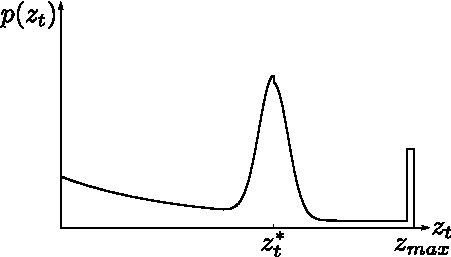
\includegraphics{beam-model.pdf}
    \caption{The probability distribution of $p(z_t | \mathbf{x}_t,\mathbf{m})$.
        The figure is based on \cite{Thrun2005}.}
    \label{fig:beam-model}
\end{figure}

However, the resulting probability distribution does not have a closed form description, which is
not a problem for particle filters, but it is for Kalman filters.

\subsection{The Distance Function based Measurement Model}\label{subsec:dt-meas-model}
The method, which enables the use of Kalman filters with laser range finder measurements on an OGM is proposed
by Dantanarayana et al. in \cite{Dantanarayana2013,Dantanarayana2016}.
In the following, this method is going to be detailed, based on \cite{Dantanarayana2016b}.

The key idea is the utilization of the distance transform (DT) operator, which is widely used in
image processing.
For a given binary image (or in this case, an OGM), the distance transform
produces an image/map (with the same size), where the value of each pixel/cell is
determined by the closest distance to any occupied pixel/cell,
by the evaluation of the distance function (DF).
If $V$ is the set of the occupied cells, and $\mathbf{x}$ is the position of an arbitrary cell on the map, then
\begin{equation}
    d_{D F}=D F(\mathbf{x})=\min _{\mathbf{v}_{\mathbf{j}} \in V}\left\|\mathbf{x}-\mathbf{v}_{\mathbf{j}}\right\|,
\end{equation}
in which an Euclidean norm is usually applied.
The distance transform then could be pre-calculated for a given map.
Figure \ref{fig:simple-dt}. shows the DT in a simplified environment,
while the DT of the OGM from Figure \ref{fig:tb3-house-ogm}. can be seen on Figure \ref{fig:gazebo-map-ogm-dt}.
\begin{figure}[htbp]
    \centering
    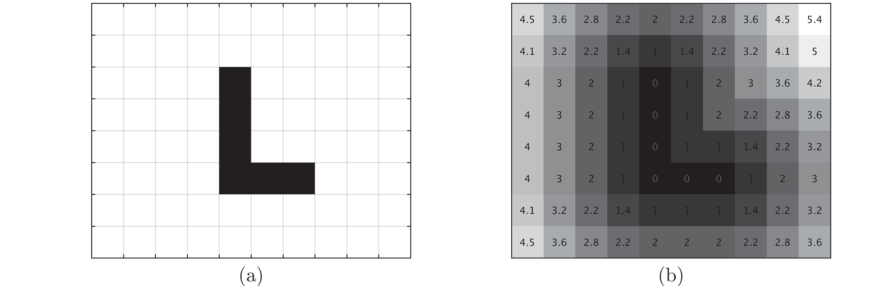
\includegraphics{simple_dt.pdf}
    \caption{A simple shape and its distance transform. Figure source: \cite{Dantanarayana2016b}.}
    \label{fig:simple-dt}
\end{figure}
\begin{figure}[htbp]
    \centering
    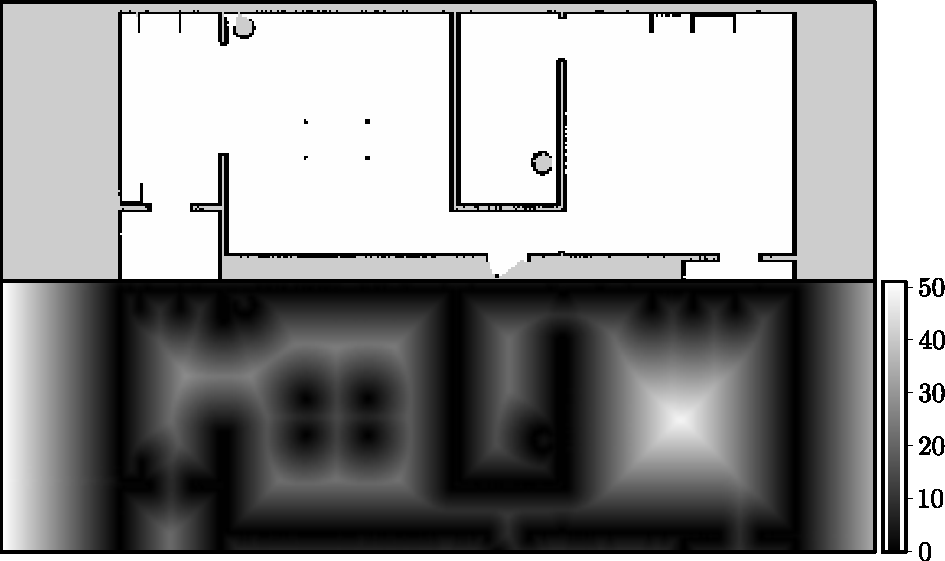
\includegraphics{dt_on_ogm.pdf}
    \caption{Part of the OGM of the TurtleBot3 House, and its distance transform.}
    \label{fig:gazebo-map-ogm-dt}
\end{figure}

Now using the LiDAR measurements, which in this case come in the form of angle-range pairs,
each detection can be transformed to map coordinates, and assigned a distance function value.
Theoretically, if the estimated pose of the robot, and the true pose of the robot aligns,
and the sensor is noiseless, each reading should indicate an occupied cell on the OGM.
Therefore, all the projected detections should have a DT of 0.
In other cases, the ray endpoints could end up on free cells, thus having a DT value larger,
than 0.

The method of transforming (projecting) the laser scans to the map, based on the estimated
location of the robot is shown in Figure \ref{fig:ogm-laser-projection}.
Mathematically, these projections are obtained as
\begin{equation}\label{eq:ray-projection}
    \mathbf{x}_{\mathrm{o}i} = \begin{bmatrix}x_{\mathrm{o}i}\\y_{\mathrm{o}i}\end{bmatrix}
    = \begin{bmatrix}x + r_i\cos(\varphi_i + \theta)\\y + r_i\sin(\varphi_i + \theta)\end{bmatrix},
\end{equation}
where the variables are according to Figure \ref{fig:ogm-laser-projection}. (the time dependency is omitted).
\begin{figure}[htbp]
    \centering
    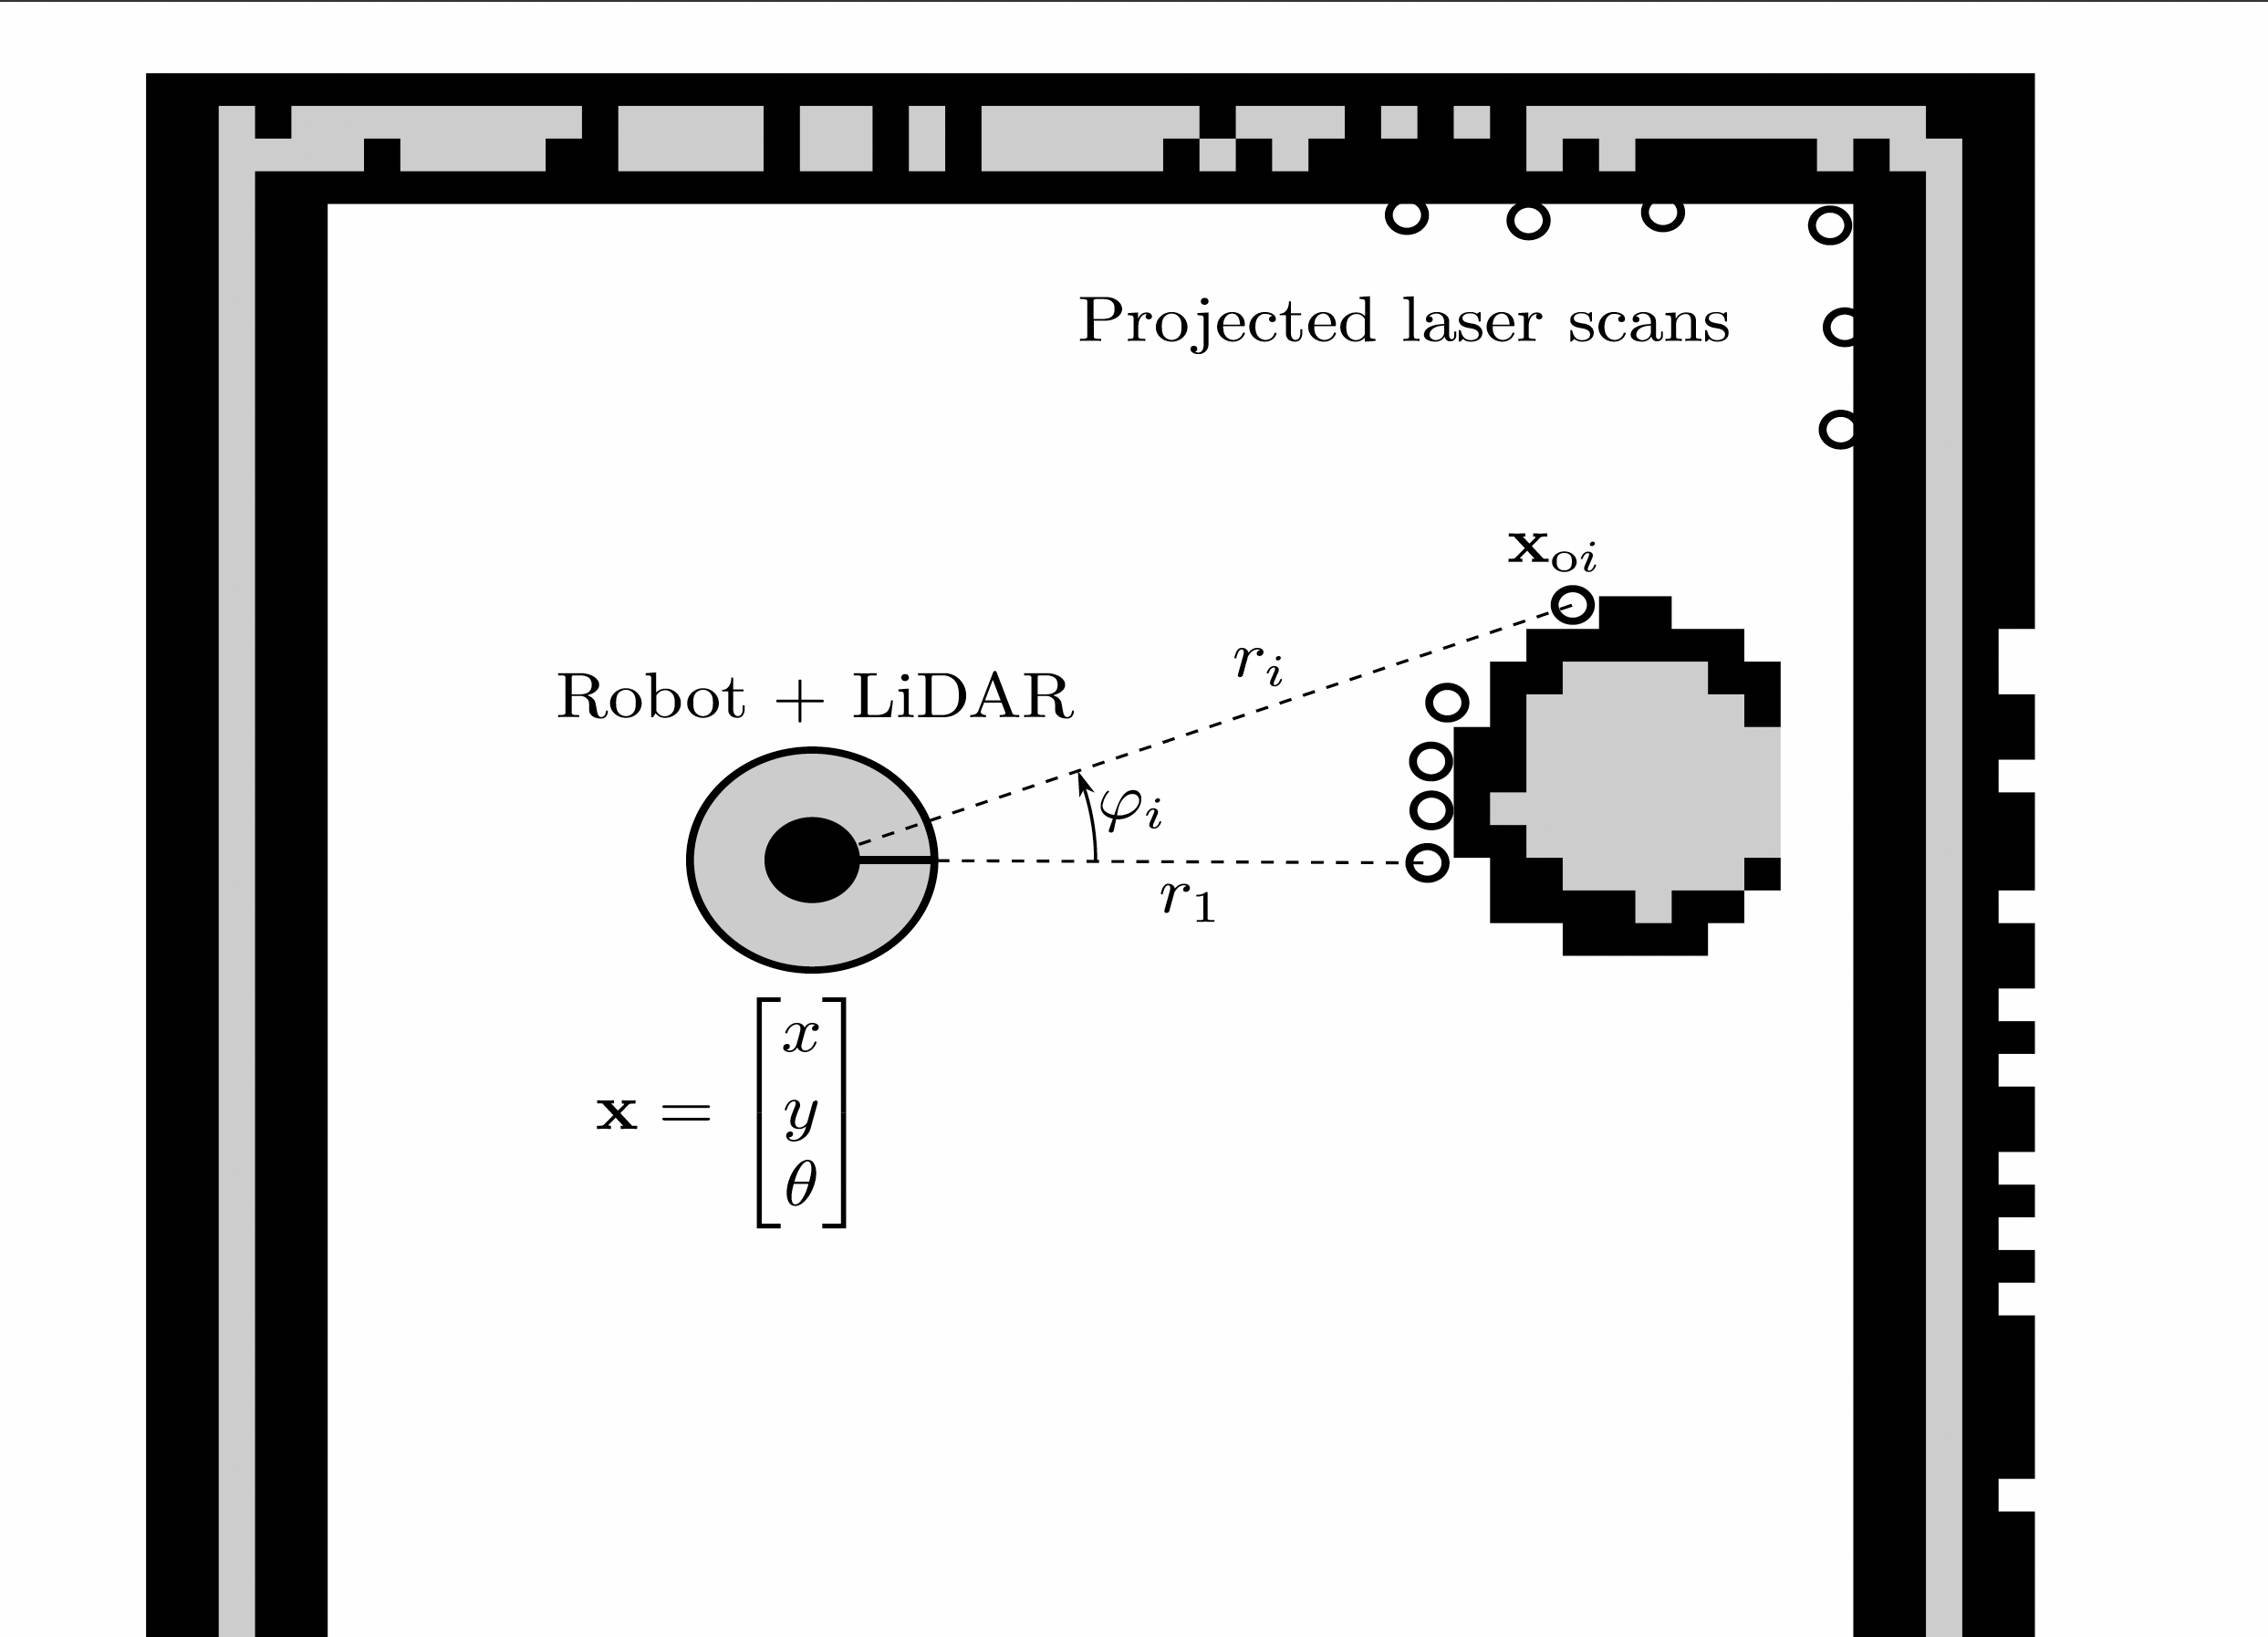
\includegraphics[width=0.8\linewidth]{dt_mapping_lidar}
    \caption{Projection of the LiDAR scans to the OGM, based on the pose of the robot.
    The rotating LiDAR emits a certain number of laser rays,
    here pictured by dashed lines for the first ray and the $i$-th ray
    (others are omitted for the sake of readability).
    The received measurement for the $i$-th ray is the length of the ray $r_i$,
    and the ray angle $\varphi_i$, measured relative from the heading of the robot,
    indicated by a thick black line.
    The ray endpoint then projected onto the map, resulting $\mathbf{x}_{\text{o}i}$ for the $i$-th ray.}
    \label{fig:ogm-laser-projection}
\end{figure}

Based on a set of measurements (for a whole revolution of the LiDAR), a vector can be constructed as follows:
\begin{equation}\label{eq:df-vector}
    \mathbf{d}_{\text{DF}} =
    \begin{bmatrix}
        DF(\mathbf{x}_{\text{o}1}) \\
        DF(\mathbf{x}_{\text{o}2}) \\
        \vdots                     \\
        DF(\mathbf{x}_{\text{o}n}) \\
    \end{bmatrix},
\end{equation}
where $n$ is the number of valid LiDAR readings for a whole revolution
(a valid reading occurs when the laser ray actually collided with an object within range, and this was
detected by the sensor).

By mapping the ray endpoints to the map, the resulting point lies
on a continuous space.
However, the distance transform of the OGM is obtained by
the distance function, which is only defined for discrete positions
on the map (the cell midpoints), not for continuous coordinates.
Instead of the quantization of the ray endpoint coordinates, a cubic spline
interpolation is applied on the distance field,
enabling the evaluation of the DF for continuous coordinates as well.
This approach also eliminates the problem of calculating the
partial derivative of the DF with respect to $x$ or $y$,
which is not defined at $x = \hat{x}, y = \hat{y}$, where
$(\hat{x}\;\; \hat{y})^{\top}$ is the coordinates of an occupied cell.
Instead, use the corresponding partial derivatives of the interpolated spline.


To obtain a single scalar value, which indicates the disparity between the projected measurements,
and the map, the Chamfer Distance (CD) is formulated. For a set of measurements,
\begin{equation}
    d_{\text{CD}} = \frac{1}{n}\sum_{i=1}^nDF(\mathbf{x}_{\text{o}i}).
\end{equation}
The CD is a good indicator for the estimation of the robot's pose: $\mathrm{CD}=0$ means
that every ray endpoint for a set of measurement at time $t$ is at the right place,
therefore the initial robot pose estimation is good.
Although, it is important to mention that this assumption does not hold in every
scenario. Consider an extreme case: for a whole revolution, the LiDAR only records
one measurement (one ray), and the OGM contains many occupied cells.
Then the CD (effectively the DT) would equal to zero at a plethora of robot poses, thus not indicating the sought true pose.
For a detailed map and sufficiently many LiDAR readings per revolution, this deficiency is minimized.

Using the CD, the measurement model is formulated as
\begin{equation}
    p(\mathbf{\mathbf{z}}_t | \mathbf{x}_t, DF_t) \sim \mathcal{F}(d_{\text{CD}t},\boldsymbol\Sigma_{\text{CDt}}),
\end{equation}
where $\mathcal{F}$ denotes the folded Gaussian distribution (this comes from the fact that the codomain of the DF is nonnegative).
The covariance is calculated as
\begin{equation}\label{eq:cd-covariance}
    \boldsymbol\Sigma_{\text{CD}} = \mathbf{J}_{\text{CD}}\mathbf{R}\mathbf{J}_{\text{CD}}^{\top},
\end{equation}
where $\mathbf{R}$ is the measurement covariance matrix, and $\mathbf{J}_{CD}$ is the Jacobian of the
Chamfer distance with respect to $\mathbf{z}_i = (\varphi_i\;\;r_i)$,
evaluated at $\mathbf{x}$.
For a LiDAR, the uncertainty of the angle measurements $\varphi_i$ is often not considered,
therefore $\mathbf{R}$ can be formulated as,
\begin{equation}\label{eq:lidar-meas-covar}
    \mathbf{R} = \sigma_r^{2}\mathbf{I}_{n\times n},
\end{equation}
where $\sigma_r$ is the standard derivation of $r_i$ (same for every ray),
and $\mathbf{I}_{n\times n}$ is the identity matrix with size $n\times n$,
if $n$ is the number of valid readings for a whole revolution of the LiDAR.
Using this simplification, the Jacobian in \eqref{eq:cd-covariance}
is only calculated with respect to $r_i$.

The observation function $\psi$ is defined as:
\begin{equation}\label{eq:observation-function}
    \psi(\mathbf{x},\mathbf{z}) = d_{\text{CD}} = \frac{1}{n}\sum_{i=1}^{n}DF(\mathbf{x}_{\text{o}i}).
\end{equation}
If the measurement $\mathbf{z}$ is not corrupted by noise, and the state $\mathbf{x}$
is at the true state (where the measurement was actually recorded), the observation
function has the value of
\begin{equation}\label{eq:impl-meas-eq}
    \psi(\mathbf{x},\mathbf{z}) = 0,
\end{equation}
forming an implicit measurement equation.


For further usages, the Jacobians of $\psi$ have to be formulated.
The Jacobian with respect to $\mathbf{x}$ is
\begin{equation}\label{eq:measmodel-jacobi-x}
    \nabla\psi_x(\mathbf{x},\mathbf{z}) := \left.\frac{\partial\psi}{\partial \mathbf{x}}\right\vert_{\mathbf{x},\mathbf{z}} =
    \frac{1}{n}
    \begin{bmatrix}
        \cfrac{1}{n}\displaystyle\sum\limits_{i=1}^{n}\left(\cfrac{\partial DF(\mathbf{x}_{\text{o}i})}{\partial x_{\text{o}}}\cfrac{\partial x_{\text{o}}}{\partial x}\right) \\
        \cfrac{1}{n}\displaystyle\sum\limits_{i=1}^{n}\left(\cfrac{\partial DF(\mathbf{x}_{\text{o}i})}{\partial y_{\text{o}}}\cfrac{\partial y_{\text{o}}}{\partial y}\right) \\
        \cfrac{1}{n}\displaystyle\sum\limits_{i=1}^{n}\left(\cfrac{\partial DF(\mathbf{x}_{\text{o}i})}{\partial x_{\text{o}}}\cfrac{\partial x_{\text{o}}(\mathbf{x},\mathbf{z}_i)}{\partial \theta}
        + \cfrac{\partial DF(\mathbf{x}_{\text{o}i})}{\partial y_{\text{o}}}\cfrac{\partial y_{\text{o}}(\mathbf{x},\mathbf{z}_i)}{\partial \theta}\right)                     \\
    \end{bmatrix}^{\top}.
\end{equation}
Here, the partial derivatives of the DF are obtained via the interpolated spline, therefore the analytical
derivation is not required.
The partial derivatives of $x_o$ and $y_o$ are trivial according to \eqref{eq:ray-projection}.

The Jacobian with respect to $\mathbf{z} = (\mathbf{z}_1\;\;\mathbf{z}_2\;\; \dots \;\; \mathbf{z}_n)^{\top}$ is simplified due to the fact that the noise effecting the
angle measurements $\varphi_i$ is neglected, therefore only the partial derivatives with respect to $r_i$ have to
be calculated:
\begin{align}\label{eq:measmodel-jacobi-z}
    \nabla\psi_z(\mathbf{x},\mathbf{z}) := \left.\frac{\partial\psi}{\partial \mathbf{z}}\right\vert_{\mathbf{x},\mathbf{z}}
     & =
    \begin{bmatrix}
        \cfrac{1}{n}\displaystyle\sum\limits_{i=1}^{n}\left(\cfrac{\partial DF(\mathbf{x}_{\text{o}i})}{\partial x_{\text{o}}}\cfrac{\partial x_{\text{o}}(\mathbf{x},\mathbf{z}_i)}{\partial r_1}
        + \cfrac{\partial DF(\mathbf{x}_{\text{o}i})}{\partial y_{\text{o}}}\cfrac{\partial y_{\text{o}}(\mathbf{x},\mathbf{z}_i)}{\partial r_1}\right) \\
        \cfrac{1}{n}\displaystyle\sum\limits_{i=1}^{n}\left(\cfrac{\partial DF(\mathbf{x}_{\text{o}i})}{\partial x_{\text{o}}}\cfrac{\partial x_{\text{o}}(\mathbf{x},\mathbf{z}_i)}{\partial r_2}
        + \cfrac{\partial DF(\mathbf{x}_{\text{o}i})}{\partial y_{\text{o}}}\cfrac{\partial y_{\text{o}}(\mathbf{x},\mathbf{z}_i)}{\partial r_2}\right) \\
        \vdots                                                                                                                                          \\
        \cfrac{1}{n}\displaystyle\sum\limits_{i=1}^{n}\left(\cfrac{\partial DF(\mathbf{x}_{\text{o}i})}{\partial x_{\text{o}}}\cfrac{\partial x_{\text{o}}(\mathbf{x},\mathbf{z}_i)}{\partial r_n}
        + \cfrac{\partial DF(\mathbf{x}_{\text{o}i})}{\partial y_{\text{o}}}\cfrac{\partial y_{\text{o}}(\mathbf{x},\mathbf{z}_i)}{\partial r_n}\right) \\
    \end{bmatrix}^{\top} \nonumber \\
     & =
    \frac{1}{n}
    \begin{bmatrix}
        \cfrac{\partial DF(\mathbf{x}_{\text{o}1})}{\partial x_{\text{o}}}\cfrac{\partial x_{\text{o}}(\mathbf{x},\mathbf{z}_1)}{\partial r_1}
        + \cfrac{\partial DF(\mathbf{x}_{\text{o}1})}{\partial y_{\text{o}}}\cfrac{\partial y_{\text{o}}(\mathbf{x},\mathbf{z}_1)}{\partial r_1} \\
        \cfrac{\partial DF(\mathbf{x}_{\text{o}2})}{\partial x_{\text{o}}}\cfrac{\partial x_{\text{o}}(\mathbf{x},\mathbf{z}_2)}{\partial r_2}
        + \cfrac{\partial DF(\mathbf{x}_{\text{o}2})}{\partial y_{\text{o}}}\cfrac{\partial y_{\text{o}}(\mathbf{x},\mathbf{z}_2)}{\partial r_2} \\
        \vdots                                                                                                                                   \\
        \cfrac{\partial DF(\mathbf{x}_{\text{o}n})}{\partial x_{\text{o}}}\cfrac{\partial x_{\text{o}}(\mathbf{x},\mathbf{z}_n)}{\partial r_n}
        + \cfrac{\partial DF(\mathbf{x}_{\text{o}n})}{\partial y_{\text{o}}}\cfrac{\partial y_{\text{o}}(\mathbf{x},\mathbf{z}_n)}{\partial r_n} \\
    \end{bmatrix}^{\top}.
\end{align}